\documentclass[11pt,aspectratio=169]{beamer}
\usepackage{fontspec}
\usepackage{amsmath,amssymb}
\usepackage{microtype}
\usepackage{booktabs}
\usepackage{pgfplots}
\pgfplotsset{compat=1.17}

% palette: dove base + dark overrides
\usecolortheme{dove}
\colorlet{mut}{white!52!black}
\colorlet{acc}{cyan!55!white}
\setbeamercolor{background canvas}{bg=black}
\setbeamercolor{normal text}{fg=white,bg=black}
\setbeamercolor{structure}{fg=white}
\setbeamercolor{frametitle}{fg=white}
\setbeamercolor{title}{fg=white}
\setbeamercolor{subtitle}{fg=mut}
\setbeamercolor{author}{fg=mut}
\setbeamercolor{date}{fg=mut}
\setbeamercolor{alerted text}{fg=acc}
\setbeamercolor{itemize item}{fg=mut}
\setbeamercolor{itemize subitem}{fg=mut}
\setbeamercolor{enumerate item}{fg=mut}

\setbeamertemplate{navigation symbols}{}
\setbeamertemplate{itemize item}{\small\raise0.15ex\hbox{\textbullet}}
\setbeamertemplate{itemize subitem}{\scriptsize\raise0.15ex\hbox{--}}
\setbeamerfont{frametitle}{size=\large,series=\bfseries}
\setbeamerfont{title}{size=\Large,series=\bfseries}

\setbeamertemplate{frametitle}{%
  \vspace{0.8em}%
  {\usebeamerfont{frametitle}\usebeamercolor[fg]{frametitle}\insertframetitle\par}%
  \vspace{0.25em}{\color{mut!45}\hrule height 0.4pt}\vspace{-0.2em}%
}
\setbeamertemplate{footline}{%
  \hbox{\begin{beamercolorbox}[wd=\paperwidth,ht=2.4ex,dp=1.4ex,leftskip=1.2em,rightskip=1.2em]{}%
    {\color{mut}\scriptsize \insertshorttitle}\hfill{\color{mut}\scriptsize\insertframenumber}%
  \end{beamercolorbox}}%
}
\setbeamertemplate{title page}{%
  \vfill{\usebeamerfont{title}\usebeamercolor[fg]{title}\inserttitle\par}
  \vspace{0.6em}{\color{mut}\normalsize\insertsubtitle\par}
  \vspace{1.6em}{\color{mut}\small\insertauthor\par}
  \vspace{0.3em}{\color{mut}\footnotesize\insertdate\par}\vfill
}

\newcommand{\Phat}{\hat P}
\newcommand{\muted}[1]{{\color{mut}#1}}

\title[PE metadata drift: re-annotation + quota sweep]{Re-annotating PE Rounds and a Metadata Quota Against Drift}
\subtitle{Experiment 2 results: per-round annotators and the $\lambda$ sweep (bioRxiv, $\varepsilon = 4$)}
\author{Kando Hsieh \quad Eli Lab, NTU}
\date{October 2026}

\begin{document}

\begin{frame}[plain]\titlepage\end{frame}

% ------------------------------------------------------------------
\begin{frame}{Setup: drift has two causes, and each needs a different tool}
MAPLE runs Private Evolution (PE) with AIM-generated metadata: each round the generator is prompted with a requested label vector, private points vote for their nearest candidate in sentence-t5 space $\varphi$, and the noisy top-$K$ survives.

\medskip
Experiment 1 located the drift in two places:
\begin{enumerate}
  \item \textbf{Generation.} The generated text does not carry the requested labels, so the requested (``inherited'') labels misdescribe the pool.
  \item \textbf{Selection.} For the \alert{blind attributes} $B = \{\texttt{word\_count}, \texttt{sample\_size}, \texttt{dominant\_data\_type}\}$ the $L_2$ vote in $\varphi$ carries almost no signal, so selection cannot pull them back.
\end{enumerate}

\medskip
This talk answers two questions:
\begin{itemize}
  \item Q1: can every round be re-labelled cheaply enough to measure and correct (1)?
  \item Q2: does forcing the survivors' marginals on $B$ toward the AIM target fix (2), and what does it cost in MAUVE?
\end{itemize}
\end{frame}

% ------------------------------------------------------------------
\begin{frame}{The generator follows requested labels only partly; Qwen and Gemini disagree on two attributes}
\textbf{Compliance}: requested AIM label vs Qwen2.5-7B label on the 14{,}000-text round-0 pool. \textbf{Annotator gap}: Qwen vs MAPLE's Gemini labels on 3{,}000 private texts.

\medskip
\centering\small
\begin{tabular}{lccc}
\toprule
attribute & compliance $\kappa$ & Qwen vs Gemini $\kappa$ & marginal JSD (Q vs G)\\
\midrule
disease\_mention         & 0.82 & 0.70 & 0.148 \\
experimental\_approach   & 0.70 & 0.61 & 0.130 \\
dominant\_data\_type     & 0.63 & 0.57 & 0.181 \\
model\_organism          & 0.62 & 0.63 & 0.170 \\
research\_goal           & 0.49 & \alert{0.29} & \alert{0.436} \\
research\_focus\_scale   & 0.47 & 0.54 & 0.131 \\
primary\_research\_area  & 0.44 & 0.49 & 0.283 \\
sample\_size             & 0.43 & \alert{0.35} & \alert{0.279} \\
\bottomrule
\end{tabular}

\raggedright
\medskip
Compliance $\kappa \in [0.43, 0.82]$: inherited labels are wrong for a large fraction of the pool, so cause (1) is real and the labels must be re-measured. For \texttt{sample\_size} and \texttt{research\_goal} the two annotators induce different label spaces; their marginals are not interchangeable.
\end{frame}

% ------------------------------------------------------------------
\begin{frame}{Re-annotation design: label once with an LLM, then distill into per-attribute classifiers}
Running Qwen every round occupies lab GPUs, and the annotator is not the object of study.
\begin{enumerate}
  \item Qwen labels the round-0 pool once (vLLM, MAPLE prompt, guided JSON over the schema, greedy; 45 texts/s).
  \item Per-attribute classifiers are trained on Qwen labels only; 70/15/15 split by prompt group.
\end{enumerate}

\medskip
Candidates, in two families:
\begin{itemize}
  \item \textbf{text encoders}: TF-IDF + logistic regression; fine-tuned SciBERT; fine-tuned BiomedBERT (both BERT-base, 3 epochs, lr $2\!\times\!10^{-5}$);
  \item \textbf{frozen embeddings + MLP}: on $\varphi$ (free, computed for the vote anyway) or on mean-pooled BiomedBERT; per-attribute or multi-head.
\end{itemize}

\medskip
Test sets: pool vs Qwen (in-domain), private vs Qwen (text gap), private vs Gemini (text + annotator gap). Private texts: evaluation only.
\end{frame}

% ------------------------------------------------------------------
\begin{frame}{Fine-tuned BiomedBERT is the per-round annotator: $\kappa = 0.83$ in-domain, 15\,s per round}
\centering\footnotesize
\resizebox{\textwidth}{!}{%
\begin{tabular}{lcccc|cc|c}
\toprule
 & \multicolumn{4}{c|}{pool test vs Qwen} & \multicolumn{2}{c|}{private vs Qwen} & private vs Gemini\\
attribute & BiomedBERT & SciBERT & TF-IDF & $\varphi$-MLP & BiomedBERT & $\varphi$-MLP & BiomedBERT\\
\midrule
dominant\_data\_type & 0.87 & 0.86 & 0.79 & 0.73 & 0.67 & 0.48 & 0.57\\
sample\_size         & 0.71 & 0.71 & 0.59 & 0.57 & 0.55 & 0.33 & 0.36\\
research\_goal       & 0.77 & 0.76 & 0.69 & 0.61 & 0.62 & 0.39 & 0.30\\
\midrule
mean (8 attributes)  & \alert{0.83} & 0.82 & 0.75 & 0.72 & \alert{0.70} & 0.53 & 0.53\\
\bottomrule
\end{tabular}}

\raggedright
\smallskip\small
\begin{itemize}
  \item Best for every attribute; SciBERT within 0.02, so PubMed pretraining barely matters. Cost: 6\,min to train all 8 heads, $\approx$15\,s to label a 14{,}000-text round.
  \item \alert{Fine-tuning is required}: frozen BiomedBERT + MLP reaches 0.73, no better than $\varphi$-MLP. Multi-head $\approx$ per-attribute ($\pm 0.02$).
  \item Real text costs 0.13 $\kappa$ (0.83 $\to$ 0.70): the classifier partly learned Qwen-generated style. Acceptable for labelling synthetic rounds. Pool-test marginal JSD 0.035 (floor 0.025).
\end{itemize}
\end{frame}

% ------------------------------------------------------------------
\begin{frame}{The blind attributes are partly absent from $\varphi$, not only ignored by the vote}
For each attribute, the gap $\Delta = \kappa_{\text{best text encoder}} - \kappa_{\text{best }\varphi\text{-MLP}}$ measures how much label information $\varphi$ fails to encode (in-domain):

\medskip
\centering\small
\begin{tabular}{lc@{\qquad}lc}
\toprule
\multicolumn{2}{c}{encoded in $\varphi$} & \multicolumn{2}{c}{partly not encoded}\\
\midrule
primary\_research\_area & 0.05 & model\_organism & 0.12\\
disease\_mention        & 0.06 & \alert{dominant\_data\_type} & \alert{0.14}\\
experimental\_approach  & 0.06 & \alert{sample\_size} & \alert{0.15}\\
                        &      & research\_goal & 0.16\\
\bottomrule
\end{tabular}

\raggedright
\medskip
Left column: a nonlinear readout of $\varphi$ recovers the label, so the $L_2$ vote is blind because other directions dominate the distance. Right column: part of the label is simply not in $\varphi$; on real text these gaps widen to 0.09--0.22.

\medskip
Consequence: any fix inside $\varphi$ (reweighting, a probe-corrected vote) is capped for $B$. A correction must use labels from outside $\varphi$, which is what the quota does.
\end{frame}

% ------------------------------------------------------------------
\begin{frame}{Quota method: rake the survivors' marginals on $B$ toward a $\lambda$-mix of AIM and MAPLE}
Round $t$: MAPLE's noisy vote gives scores $s_i$ and its top-$K$; let $R_{t,k}$ be the marginal of attribute $k \in B$ in that top-$K$, and $\Phat_k$ the marginal of the AIM $\varepsilon{=}4$ records (post-processing, no extra privacy cost). Target per attribute:
\[
  m_k(v) \;\propto\; \Phat_k(v)^{\lambda}\; R_{t,k}(v)^{1-\lambda}, \qquad \lambda \in [0,1].
\]

\vspace{-0.3em}
\begin{enumerate}
  \item \textbf{Raking.} Joint-cell weights $w_c$ over $B$-cells start from $R_t$ (+5\% of the candidate composition), then iterative proportional fitting matches all $m_k$. A cell that runs out of candidates is frozen at its supply; its deficit goes to other cells.
  \item \textbf{Rounding.} Quotas $K_c$ by largest remainder, $\sum_c K_c = K$.
  \item \textbf{Selection.} Inside each cell, keep the $K_c$ highest-vote candidates; leftovers filled by global vote order.
\end{enumerate}

\medskip
$\lambda = 0$ reproduces MAPLE's top-$K$; $\lambda = 1$ targets the AIM marginals. The first version used joint cells (29 most frequent + \texttt{\_\_other\_\_}); it put 47\% of the AIM mass into \texttt{\_\_other\_\_}, where the quota has no effect, hence raking on one-way marginals.
\end{frame}

% ------------------------------------------------------------------
\begin{frame}{Sweep setup: $\lambda \times$ in-loop annotator, evaluated with Qwen}
\textbf{PE}: bioRxiv, MAPLE settings at $\varepsilon = 4$: $T = 4$ iterations, $\sigma = 2.58$, $K = 2000$, $L = 6$. Round 0 reuses one shared pre-vote pool, so all runs start from the same candidates; 5 vote+select steps, 12{,}000 variations per later round.

\medskip
\textbf{In-loop labels} (what the quota sees); \texttt{word\_count} is always measured:
\begin{itemize}
  \item \texttt{inherited}: requested AIM labels (MAPLE's own);
  \item \texttt{classifier}: fine-tuned BiomedBERT for \texttt{sample\_size}, \texttt{dominant\_data\_type};
  \item \texttt{qwen}: the evaluation annotator itself, i.e. an oracle-style upper reference.
\end{itemize}

\medskip
\textbf{Grid}: $\lambda \in \{0, 0.25, 0.5, 0.75, 1\}$, constant schedule; linear $\lambda_t = \lambda t/T$ at the end of the queue; seed 1 for a subset. 26 runs, $\approx$45\,min each, 3 GPUs.

\medskip
\textbf{Metrics} on the $K$ survivors: MAUVE (sentence-t5, vs 2{,}000 test texts); per-attribute JSD vs the Qwen-labelled test set; blind mean over $B$, other mean over the remaining 6.
\end{frame}

% ------------------------------------------------------------------
\begin{frame}{MAPLE drifts on the blind attributes while MAUVE stays flat}
MAPLE ($\lambda = 0$), JSD vs Qwen-labelled test set:

\medskip
\centering\small
\begin{tabular}{lccc}
\toprule
 & round 0 & round 4 & change\\
\midrule
blind JSD mean ($B$)    & 0.187 & \alert{0.274} & $+0.087$\\
\quad \texttt{word\_count} & 0.21 & \alert{0.48} & $+0.27$\\
MAUVE                   & $\approx 0.63$ & 0.632 & $\approx 0$\\
\bottomrule
\end{tabular}

\raggedright
\medskip
\begin{itemize}
  \item The drift predicted in Experiment 1 is present in the real run: four rounds of selection push the blind marginals away from the private data.
  \item \alert{Length dominates}: \texttt{word\_count} JSD more than doubles. The vote favours one length band and nothing in $\varphi$-distance resists it.
  \item MAUVE does not register the drift. A metric computed in the vote's embedding cannot see what the vote cannot see; attribute JSD has to be reported alongside it.
\end{itemize}
\end{frame}

% ------------------------------------------------------------------
\begin{frame}{Round-4 results across $\lambda$ and in-loop annotators}
\centering\small
\resizebox{\textwidth}{!}{%
\begin{tabular}{lcc|c|ccc}
\toprule
setting & MAUVE $\uparrow$ & blind JSD $\downarrow$ & other JSD $\downarrow$ & word\_count & dom.\_data\_type & sample\_size\\
\midrule
MAPLE ($\lambda{=}0$)       & 0.632 & 0.274 & 0.109 & 0.483 & 0.210 & 0.129\\
classifier $\lambda{=}0.25$ & 0.760 & 0.234 & 0.101 & 0.367 & 0.180 & 0.156\\
classifier $\lambda{=}0.5$  & \alert{0.777} & 0.177 & \alert{0.094} & 0.236 & 0.123 & 0.172\\
classifier $\lambda{=}0.75$ & 0.725 & 0.140 & 0.097 & 0.128 & \alert{0.098} & 0.194\\
classifier $\lambda{=}1$    & 0.625 & \alert{0.122} & 0.117 & 0.060 & 0.104 & 0.202\\
inherited $\lambda{=}1$     & 0.786 & 0.138 & 0.097 & 0.062 & 0.222 & 0.130\\
qwen $\lambda{=}1$          & 0.710 & 0.169 & 0.110 & 0.062 & 0.158 & 0.288\\
\midrule
floor JSD$(\Phat_k, \text{Qwen test})$ & -- & -- & -- & 0.062 & 0.158 & 0.285\\
\bottomrule
\end{tabular}}

\raggedright
\medskip
Means over seeds where two exist (MAPLE, classifier $\lambda \in \{0.5, 1\}$, qwen $\lambda{=}1$). The floor is the JSD between the AIM target and the Qwen-labelled test set: a quota that hits $\Phat_k$ exactly cannot score below it.
\end{frame}

% ------------------------------------------------------------------
\begin{frame}{Length is solved, data type needs re-annotation, sample size is unreadable}
\textbf{\texttt{word\_count}} (measured, no annotator). 0.483 $\to$ \alert{0.060} (the floor) at $\lambda = 1$, any annotator. Supply does not bind (variation prompts request a length), so no refill is needed.

\smallskip
\textbf{\texttt{dominant\_data\_type}}. Re-annotated labels halve the JSD (0.210 $\to$ 0.098, classifier $\lambda{=}0.75$); inherited labels leave it at 0.20--0.22, since with compliance $\kappa = 0.63$ the quota balances requested labels, not content. Inherited's low blind mean comes from length alone: \alert{content attributes need re-annotation}.

\smallskip
\textbf{\texttt{sample\_size}}. qwen $\lambda{=}1$ lands at 0.288, the floor 0.285: the quota succeeds in matching $\Phat_k$, but $\Phat_k$ lives in Gemini/AIM label space and the labels in Qwen space ($\kappa = 0.35$ between them). JSD vs the Qwen test set then measures annotator mismatch, not drift. Fix: translate the target
\[
  \Phat^{\text{Qwen}}_k = C^\top \Phat^{\text{Gemini}}_k, \qquad C_{uv} = \Pr(\text{Qwen}=v \mid \text{Gemini}=u),
\]
$C$ from the 3{,}000 private texts labelled by both; then rerun.
\end{frame}

% ------------------------------------------------------------------
\begin{frame}{$\lambda \approx 0.5$--$0.75$ dominates MAPLE; $\lambda = 1$ has collateral cost}
\begin{columns}[T]
\begin{column}{0.47\textwidth}
\centering
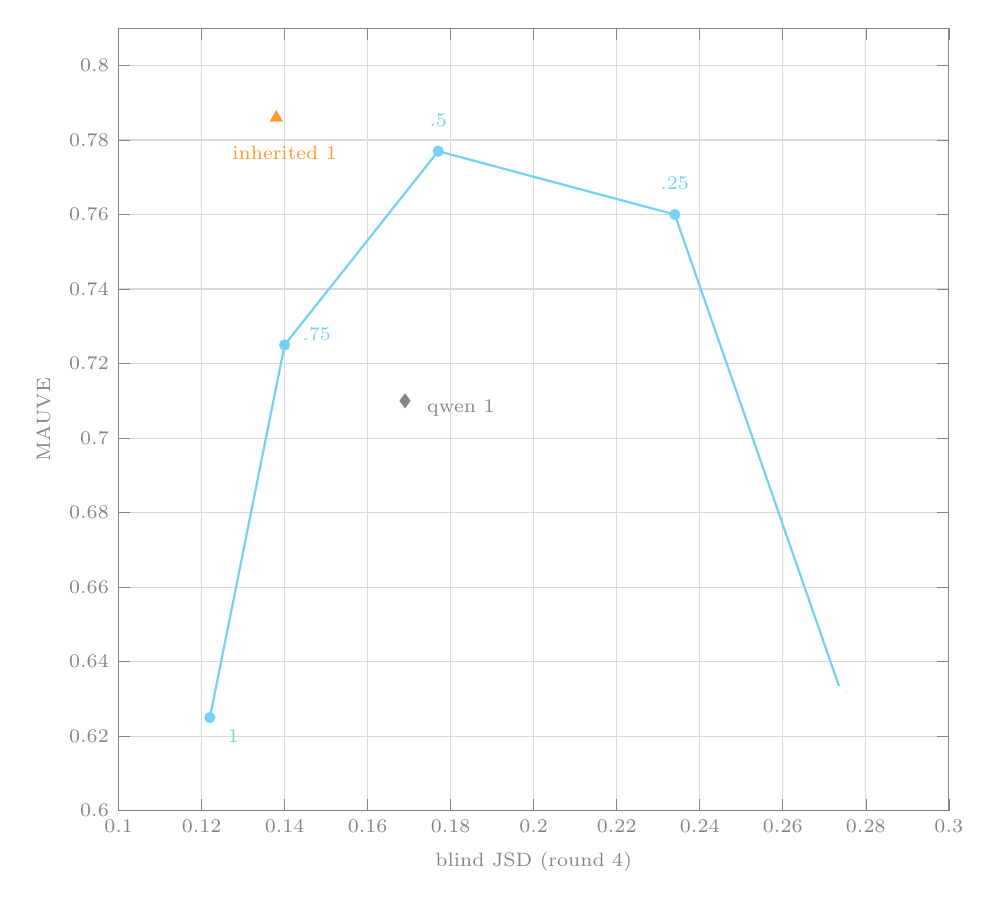
\begin{tikzpicture}
\begin{axis}[
  width=\linewidth, height=0.95\linewidth,
  xlabel={blind JSD (round 4)}, ylabel={MAUVE},
  xmin=0.10, xmax=0.30, ymin=0.60, ymax=0.81,
  axis line style={mut}, tick style={mut}, every tick label/.append style={font=\scriptsize, color=mut},
  label style={font=\scriptsize, color=mut},
  grid=major, grid style={mut!30},
]
\addplot[acc, thick, mark=*, mark size=1.6pt] coordinates {(0.274,0.632) (0.234,0.760) (0.177,0.777) (0.140,0.725) (0.122,0.625)};
\addplot[only marks, white, mark=square*, mark size=1.8pt] coordinates {(0.274,0.632)};
\addplot[only marks, orange!80!white, mark=triangle*, mark size=2.4pt] coordinates {(0.138,0.786)};
\addplot[only marks, mut, mark=diamond*, mark size=2.4pt] coordinates {(0.169,0.710)};
\node[font=\scriptsize, white, anchor=north east] at (axis cs:0.276,0.628) {MAPLE};
\node[font=\scriptsize, acc, anchor=south] at (axis cs:0.234,0.764) {.25};
\node[font=\scriptsize, acc, anchor=south] at (axis cs:0.177,0.781) {.5};
\node[font=\scriptsize, acc, anchor=west] at (axis cs:0.142,0.728) {.75};
\node[font=\scriptsize, acc, anchor=west] at (axis cs:0.124,0.620) {1};
\node[font=\scriptsize, orange!80!white, anchor=north] at (axis cs:0.140,0.781) {inherited 1};
\node[font=\scriptsize, mut, anchor=west] at (axis cs:0.172,0.708) {qwen 1};
\end{axis}
\end{tikzpicture}

\muted{\scriptsize teal: classifier, labels = $\lambda$}
\end{column}
\begin{column}{0.51\textwidth}
\small
\begin{itemize}
  \item Classifier $\lambda \in [0.5, 0.75]$: MAUVE 0.73--0.78 vs 0.63 and blind JSD 0.14--0.18 vs 0.27; other attributes equal or better (0.094--0.097 vs 0.109).
  \item At $\lambda = 1$ MAUVE falls back to 0.63 and non-blind attributes degrade (\texttt{disease\_mention} 0.042 $\to$ 0.084, \texttt{experimental\_approach} 0.084 $\to$ 0.117): correlated attributes get pulled along, and more low-vote texts survive.
  \item Linear schedule $\lambda_t = \lambda t/T$: lower MAUVE at equal $\lambda$. Constant is kept.
\end{itemize}
\end{column}
\end{columns}
\end{frame}

% ------------------------------------------------------------------
\begin{frame}{Open issues before the gain can be claimed}
\begin{itemize}
  \item \textbf{Variance.} Two seeds exist for MAPLE, classifier $\lambda \in \{0.5, 1\}$, qwen $\lambda{=}1$, but the seed spread has not been read. The MAUVE gain needs error bars first.
  \item \textbf{Label space.} Translate $\Phat_k$ into the loop/eval annotator's space with $C$, rerun \texttt{sample\_size}; without it annotators cannot be compared on that attribute.
  \item \textbf{Which annotator is right.} For \texttt{sample\_size} and \texttt{research\_goal}, no classifier trained on Qwen labels agrees with Gemini beyond Qwen's own $\kappa$ (0.35, 0.29). A human spot check on $\sim$100 texts would settle the reference.
  \item \textbf{Self-annotation.} Qwen labels its own generations; Gemini labels on the synthetic pool (API key pending) would remove this.
  \item \textbf{Metric.} MAUVE is in-loop (same $\varphi$ as the vote); add an out-of-loop text metric.
  \item \textbf{Coverage.} GPUs idled 21:31 $\to$ 12:00. Next queue: $\varepsilon \in \{2, 1\}$ and more seeds.
\end{itemize}
\end{frame}

% ------------------------------------------------------------------
\begin{frame}{Takeaway}
\begin{itemize}
  \item The generator follows requested labels only partly, so drift must be measured with fresh labels; a fine-tuned BiomedBERT supplies them at $\kappa = 0.83$ for 15\,s per round.
  \item MAPLE's blind-attribute JSD grows 0.19 $\to$ 0.27 over four rounds, mostly length, invisible to MAUVE.
  \item A raked quota toward the AIM marginals with $\lambda \approx 0.5$--$0.75$ lowers blind JSD to 0.14--0.18 and raises MAUVE to 0.73--0.78, pending seed variance.
  \item \texttt{sample\_size} remains open until target and labels share one annotator space.
\end{itemize}
\end{frame}

\end{document}
